%% When Do Graph Neural Networks Help in Cross-Sectional Stock Ranking?
%% ICAIF 2026 -- ACM SIGCONF (acmart). Compiles on Overleaf (acmart built in).
%% Build: pdflatex -> bibtex -> pdflatex x2  (or latexmk -pdf main.tex)
%% Figures: PDF masters live in ../figures/ (see \graphicspath below).
%% This .tex is the SUBMISSION version derived from docs/storya_paper_draft_v2.md:
%% provenance source-citations, editor notes and red-line boxes were dropped; every
%% number here is traceable to that working draft and its source CSVs.

\documentclass[sigconf,nonacm]{acmart}

\usepackage{booktabs}
\usepackage{graphicx}
\usepackage{amsmath}
\graphicspath{{../figures/}{figures/}}

%% --- ICAIF 2026 metadata (fill camera-ready values) ---
\acmConference[ICAIF '26]{ACM International Conference on AI in Finance}{November 2026}{Singapore}
\acmYear{2026}
\copyrightyear{2026}
\setcopyright{none}

\begin{document}

\title{When Do Graph Neural Networks Help in Cross-Sectional Stock Ranking?}
\subtitle{A Multi-Seed, Multi-Universe, Cost-Aware Study of the US S\&P~500}

%% TODO: fill author / affiliation for camera-ready.
\author{Anonymous Author(s)}
\affiliation{%
  \institution{Affiliation}
  \city{City}
  \country{Country}}
\email{author@example.edu}

\renewcommand{\shortauthors}{Anonymous}

\begin{abstract}
Graph neural networks (GNNs) are widely reported to improve cross-sectional stock ranking by encoding inter-stock relations as graph edges, yet these gains are almost always quoted as single-seed, single-split numbers without multiple-comparison defence. We ask a narrower and more reproducible question, namely \emph{when}, if ever, a graph helps, and answer it under a deliberately strict protocol. We evaluate a tuned model ladder, running from a gradient-boosted-tree baseline up to a heterogeneous relational GNN (rungs L0--L7), over twelve expanding quarterly walk-forward folds and ten random seeds on the US S\&P~500, with two pre-registered confirmatory families. The first family asks whether \emph{any} tuned model beats a tuned LightGBM benchmark. Hansen's Superior Predictive Ability test fails to reject this null in both feature universes ($p=0.277$ and $p=0.077$); because that comparison is itself underpowered, this is a fail-to-reject rather than a claim of equality. Local Diebold--Mariano ladder rungs show that the neural lift that does exist comes from a non-graph multilayer perceptron rather than from the graph: in the richer universe the tuned MLP beats LightGBM (local $\Delta$IC${}=+0.015$), whereas adding a correlation-graph attention network loses to that MLP ($\Delta$IC${}=-0.012$). The second family isolates the \emph{causal} effect of each edge type at a frozen network capacity; none of six edge contrasts survives Benjamini--Hochberg control, and all six are underpowered. A net-of-cost crosswalk confirms that the two load-bearing Universe-C rungs survive a 10\,bps cost, while the one IC rung that does not carry to net economics, the tuned news-edge arm underperforming the correlation-GAT, is a near-zero, fold-fragile difference that the capacity-matched causal test does not echo. We frame these as conditional findings and failure modes, and contribute a reusable evaluation scaffold for GNN-finance work.
\end{abstract}

\begin{CCSXML}
<ccs2012>
<concept>
<concept_id>10010147.10010257</concept_id>
<concept_desc>Computing methodologies~Machine learning</concept_desc>
<concept_significance>500</concept_significance>
</concept>
</ccs2012>
\end{CCSXML}
\ccsdesc[500]{Computing methodologies~Machine learning}

\keywords{cross-sectional stock ranking, graph neural networks, walk-forward evaluation, Hansen SPA, multiple-comparison control, transaction costs}

\maketitle

\section{Introduction}\label{sec:intro}

\emph{Cross-sectional stock ranking} is the task of predicting, every trading day, the \emph{relative} order of next-period returns across a fixed universe of stocks, here the constituents of the US S\&P~500. A model that orders the top decile correctly yields a tradeable dollar-neutral long-short portfolio; a model that ranks no better than chance loses to transaction costs. The standard quality metric is the \emph{Information Coefficient} (IC), the cross-sectional Spearman rank correlation between predicted scores and realised forward returns, averaged over test days.

Recent GNN papers, most prominently Feng et al.~\cite{feng2019temporal} on temporal relational ranking, Kim et al.~\cite{kim2019hats} on HATS, and Sawhney et al.~\cite{sawhney2021sthansr} on STHAN-SR, report sizeable IC gains by encoding inter-stock relations (sector membership, Wikidata ontologies, news co-mentions) as graph edges and applying message passing. These headline gains are almost always quoted as \emph{single-seed} and \emph{single-split} numbers. Three concerns motivate a closer and more disciplined look.

First, \textbf{single-seed inflation and cross-seed dispersion} are large in this regime. Even after tuning and seed-averaging, the per-arm 95\% bootstrap CIs here are as wide as the IC point estimates themselves: the Universe-C correlation-GAT pooled IC of $0.0224$ carries a 95\% CI of $[-0.0080,+0.0559]$, so a single-seed, single-split number can land almost anywhere in that band. Re-tuning hyperparameters does not remove this dispersion; only multi-seed evaluation surfaces it. Second, \textbf{regime concentration}: cross-sectional ranking profit is episodic, and a single high-dispersion quarter can dominate an annual number, so a positive pooled IC can be the artefact of one good quarter unless per-fold behaviour is disclosed. Third, \textbf{capacity confounding}: when each model rung is independently tuned under an equal compute budget, an edge ablation that compares differently-sized networks confounds ``did the edge help'' with ``did the bigger network help'', so a clean causal read of an edge requires holding capacity fixed.

We address all three with a single tuned ladder and two \emph{separate} pre-registered confirmatory families. The \textbf{predictive family} (Family-1) asks the model-selection question, does any tuned arm beat a tuned LightGBM, using Hansen's Superior Predictive Ability (SPA) test~\cite{hansen2005spa} over nine candidates, with Diebold--Mariano / Harvey--Leybourne--Newbold (DM/HLN) pairwise tests~\cite{diebold1995comparing,harvey1997testing} under Benjamini--Hochberg (BH) false-discovery-rate control~\cite{benjamini1995controlling} as local evidence. The \textbf{causal family} (Family-2) freezes the full hyperparameter vector of the correlation-graph operating point and varies \emph{only} the edge set, so the matched $\Delta$IC isolates the pure edge effect at fixed capacity. Figure~\ref{fig:pipeline} summarises the pipeline.

\begin{figure*}[t]
  \centering
  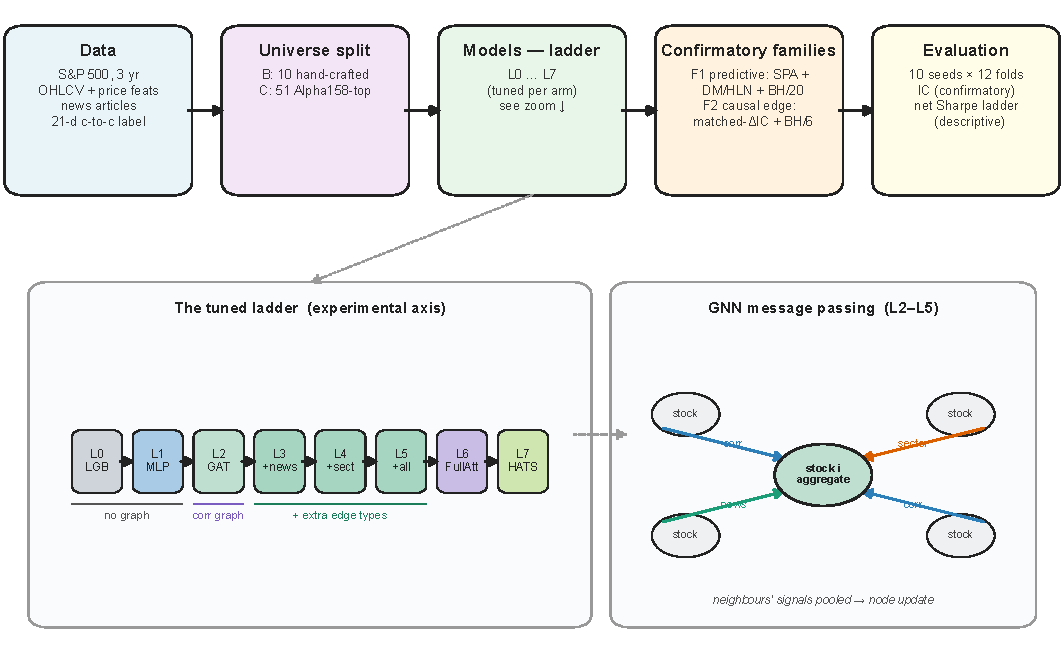
\includegraphics[width=\textwidth]{pipeline_confirmatory}
  \caption{End-to-end confirmatory pipeline. Raw daily OHLCV for the S\&P~500 $\rightarrow$ per-day cross-sectional feature matrix (Universe~B, 10 hand-crafted dimensions; or Universe~C, 51 Alpha158 columns) $\rightarrow$ graph snapshot (rolling-correlation edges, optionally augmented with GICS-sector or point-in-time news co-occurrence edges) $\rightarrow$ one rung of the tuned L0--L7 ladder $\rightarrow$ cross-sectional ranking $\rightarrow$ top-decile equal-weight dollar-neutral long-short portfolio rebalanced every 21 trading days $\rightarrow$ evaluation by pooled IC, the two confirmatory families, and a descriptive gross/net cost crosswalk.}
  \label{fig:pipeline}
\end{figure*}

\paragraph{Two feature universes.} Both universes use the \emph{same set of stocks} and differ only in the features each stock carries. \textbf{Universe~B} is a 10-dimensional minimalist hand-crafted set built from price and volume alone (windowed return means and standard deviations at 5/10/21 days, 12-month momentum, an extreme-return statistic, dollar volume, and a 5-day rolling correlation); the ``B'' stands for \emph{baseline}. \textbf{Universe~C} is a 51-dimensional subset of Qlib's Alpha158 factor library~\cite{yang2020qlib} (top-15 factor groups by the project's earlier ranking); the ``C'' stands for \emph{composite}. All values are taken strictly at $T-1$. We compare two universes of very different richness to test whether GNN advantage depends on how strong the node features already are.

\paragraph{Headline findings.} No tuned arm is confirmed to beat tuned LightGBM: Hansen SPA does not reject in either universe (Universe~B $p_{\text{consistent}}=0.277$, Universe~C $p_{\text{consistent}}=0.077$), and the vs-LightGBM comparison is underpowered (observed gaps below the 80\% minimum detectable effect), so this is a fail-to-reject, not evidence of equality. The neural lift that exists is carried by the non-graph MLP rather than the graph: in Universe~C the tuned MLP beats tuned LightGBM (L1$-$L0 $\Delta$IC${}=+0.0148$, HLN $p=0.011$, BH-reject) while adding a correlation-graph attention layer loses to that MLP (L2$-$L1 $\Delta$IC${}=-0.0119$, $p=6.9\times10^{-6}$, BH-reject); both are \emph{local} ladder rungs, not global SPA wins. The causal edge family finds \textbf{0/6} contrasts surviving BH-FDR and \textbf{6/6} underpowered. Under a net-of-cost convention, the two load-bearing Universe-C rungs hold at 10\,bps, while the one IC rung that flips convention (the tuned news-edge arm underperforming corr-GAT on ranking) is a near-zero, fold-fragile net difference, flagged cost-sensitive and not echoed by the capacity-matched causal test. We frame these as \emph{conditional findings} and \emph{failure modes}, not architecture-supremacy claims.

\section{Related Work}\label{sec:related}

\paragraph{GNN baselines for stock ranking.} Feng et al.~\cite{feng2019temporal} frame stock prediction as learning-to-rank over industry and Wikidata relation graphs with a temporal graph-convolution, reporting IC and return on a single split. Kim et al.~\cite{kim2019hats} introduce HATS, a hierarchical graph-attention network over 75 Wikidata relation types; it is the blueprint for our HATS-3R-adapt rung (L7), which restricts the relations to correlation, GICS sector, and news co-occurrence and switches the head to 21-day cross-sectional ranking. Cheng and Li~\cite{cheng2021adgat} (AD-GAT) infer dynamic firm relations through an unmasked attention mechanism, and Li et al.~\cite{li2024master} (MASTER) alternate intra- and inter-stock attention; both represent the \emph{dense learned-attention} family that our L6 rung stands in for. Sawhney et al.~\cite{sawhney2021sthansr} re-frame selection as ranking over a spatiotemporal hypergraph, and Lin et al.~\cite{lin2021tra} (TRA) route samples to pattern-specific predictors. The common thread is rich relational structure evaluated under single-seed, single-split conditions.

\paragraph{Methodology-leaning quantitative finance.} Hou, Xue and Zhang~\cite{hou2020replicating} replicate 452 cross-sectional anomalies under a uniform protocol and find 65\% fail multiple-comparison-corrected replication; we adopt that discipline. L\'opez de Prado~\cite{lopezdeprado2018advances} codifies block bootstrap and purge-and-embargo cross-validation, which we use throughout. Hansen~\cite{hansen2005spa} supplies the SPA test, with Politis and Romano~\cite{politis1994stationary} providing its stationary bootstrap and Newey and West~\cite{newey1987simple} the HAC standard errors.

\paragraph{Position relative to prior work.} To our knowledge this is the first study to combine, on the S\&P~500, all of: 10 seeds $\times$ 12-fold expanding walk-forward $\times$ a tuned model ladder $\times$ two separate pre-registered confirmatory families (predictive SPA/DM-HLN \emph{and} capacity-matched causal edge attribution) $\times$ a gross/net cost ladder $\times$ point-in-time news handling $\times$ explicit disclosure of a tuned-config stability failure. Table~\ref{tab:related} makes the gap explicit; the entries reflect each work's \emph{reported} evaluation protocol, and ``$\times$'' marks a property the paper does not report, not a claim that the property is impossible.

\begin{table*}[t]
  \centering
  \caption{Related-work evaluation matrix. Entries reflect each work's reported protocol; $\times$ = not reported (not a claim of impossibility).}
  \label{tab:related}
  \begin{tabular}{@{}llllccc@{}}
    \toprule
    Work & Venue/Year & Graph / relation & Test design & Multi-seed & SPA/DM-FDR & Cost ladder \\
    \midrule
    Feng et al.~\cite{feng2019temporal}      & TOIS 2019  & industry + Wikidata          & single split & $\times$ & $\times$ & $\times$ \\
    Kim et al.~\cite{kim2019hats}            & 2019       & 75 Wikidata relations        & single split & $\times$ & $\times$ & $\times$ \\
    Cheng \& Li~\cite{cheng2021adgat}        & AAAI 2021  & unmasked learned attention   & single split & $\times$ & $\times$ & $\times$ \\
    Sawhney et al.~\cite{sawhney2021sthansr} & AAAI 2021  & spatiotemporal hypergraph    & single split & few      & $\times$ & $\times$ \\
    Lin et al.~\cite{lin2021tra}             & KDD 2021   & temporal routing (no graph)  & single split & $\times$ & $\times$ & $\times$ \\
    Li et al.~\cite{li2024master}            & AAAI 2024  & market-guided attention      & single split & $\times$ & $\times$ & $\times$ \\
    Chen et al.~\cite{finmamba2025}          & 2025       & dynamic pruned graph + Mamba & single split & $\times$ & $\times$ & profit only \\
    \textbf{This work}                       & ---        & tuned corr/sector/news ladder + FC edge arm & 12-fold WF & \textbf{10} & \textbf{SPA+DM+FDR} & \textbf{0--30\,bps} \\
    \bottomrule
  \end{tabular}
\end{table*}

\section{Methodology}\label{sec:method}

\subsection{Walk-forward cross-validation}
We use a 12-fold \emph{expanding-window walk-forward}: for fold $k$ the training set is all data up to a quarter boundary, the validation set is the next quarter, and the test set is the quarter after that. The twelve test quarters span 2023\,Q1 through 2025\,Q4, giving $T=749$ pooled test days. Because the label is a 21-day forward return, we drop the final 21 trading days of each training set (a \emph{purge embargo}) to eliminate label overlap~\cite{lopezdeprado2018advances}. A secondary sliding-252-day axis is reported as robustness only and carries no independent inference.

\subsection{Information coefficient and portfolio}
Daily IC is the cross-sectional Spearman rank correlation between predictions and next-day 21-day-forward returns over all stocks with non-missing features that day; headline IC is the pooled mean over all test days across all 12 folds. We use Spearman because rank IC is invariant to monotonic transforms and is the factor-investing convention. Each day we sort by predicted score, long the top $K$ and short the bottom $K$ with $K=\lfloor 10\%\times n_{\text{valid}}\rfloor$, equal-weight and dollar-neutral, rebalanced every 21 trading days. The long-short Sharpe is annualised by $\sqrt{252/21}$. \emph{Net} Sharpe subtracts a one-way transaction cost at $\{0,5,10,15,20,30\}$\,bps per rebalance (net${}={}$gross${}-{}$turnover$_{\text{L1}}\times\text{bps}/10^4$), with the headline level at 10\,bps; net Sharpe is reported only as a descriptive economic-sensitivity layer.

\subsection{Two confirmatory families}\label{sec:families}
We ask two different questions and keep them statistically separate. \emph{Did any model win?} is a model-selection question answered against multiple candidates (Family-1). \emph{Did this specific edge cause an improvement?} is a controlled-intervention question answered by changing only the edge while holding everything else fixed (Family-2).

\textbf{Family-1 (predictive).} The benchmark is the tuned LightGBM rung (L0); the candidates are the nine other tuned rungs. We run Hansen SPA (consistent variant, loss${}={}-$daily IC, stationary block bootstrap, block${}=21$\,d) to ask whether the best of the $M=9$ candidates beats the benchmark after accounting for selection. As local evidence we run DM/HLN paired tests on a pre-registered family of 20 contrasts, five ladder rungs $\{$L1$-$L0, L2$-$L1, L6$-$L2, L7$-$L2, L2s$-$L2$\}$ and five edge-DAG rungs $\{$L3$-$L2, L4$-$L2, L5$-$L2, L5$-$L4, L5$-$L3$\}$, in each of the two universes, under BH-FDR at $q=0.05$. The DM statistic uses Newey--West HAC standard errors~\cite{newey1987simple}; the HLN factor $\sqrt{(T+1-2h+h(h-1)/T)/T}$ with $h=21$ corrects the small $T/h$ ratio.

\textbf{Family-2 (causal).} The capacity confound means a tuned-vs-tuned edge comparison is not a clean edge effect. We add fixed-capacity (FC) arms that run L3/L4/L5's edge sets at the frozen tuned hyperparameter vector of L2, varying \emph{only} the edge set. The matched $\Delta$IC isolates the pure edge effect at the L2 operating point. Inference is the paired fold-level seed-averaged $\Delta$IC over $n\approx12$ fold blocks, block bootstrap over folds, and BH-FDR over the six contrasts; the per-row CIs are unadjusted descriptive intervals.

\textbf{Power.} For every contrast we report a minimum detectable effect $\text{MDE}=2.8\times\text{SE}_{\text{block}}$ with $n_{\text{eff}}=T_{\text{days}}/21$, so that fail-to-reject can be distinguished from no-effect.

\subsection{Pre-registration}
The frozen protocol and the frozen tuned hyperparameters (md5 \texttt{59ddd0a2}) were committed before the confirmatory launch. The two confirmatory families are the \emph{only} inferential families; all prior work (horizon ablation, the loss-function horse race, the Plan-AAA factor ranking) is flagged exploratory and is disclosed but never allowed to count as confirmatory evidence. Net Sharpe is a descriptive layer; IC remains the sole confirmatory metric, and no third BH-FDR family is opened on Sharpe.

\section{Data and Setup}\label{sec:data}

The universe is the S\&P~500 constituents as of each trading day; frequency is daily close-to-close. The label is the next-day cross-sectionally $z$-scored 21-day forward log return, locked across all experiments. Ten canonical seeds are used everywhere. Each ladder rung changes exactly one design choice relative to the rung below it (Table~\ref{tab:ladder}); every rung is independently tuned under an equal compute budget (Optuna, $N=30$ trials per arm). Graph $\alpha$1 is a 126-day rolling Spearman correlation (edge if $|\rho|>0.6$, refreshed every 21 days from training data only); $\alpha$2 is static GICS sector connectivity; news edges are point-in-time (two stocks share an edge on day $T$ if co-mentioned in an article published before NYSE close of $T-1$); $\alpha$4 stacks all three. The confirmatory budget is 2160 main cells (9 non-HATS arms $\times$ 2 universes $\times$ 12 folds $\times$ 10 seeds), 240 L7/HATS cells, and 720 Family-2 fixed-capacity cells; each store is internally complete (0 failed, 0 duplicate \texttt{cell\_id}) and consumed by its respective family. Models are GAT~\cite{velickovic2018gat}, GraphSAGE-Mean~\cite{hamilton2017graphsage}, an MLP, and LightGBM; the L7 per-relation parameterisation follows R-GCN~\cite{schlichtkrull2018rgcn}; SPA is computed with the \texttt{arch} package~\cite{sheppard_arch}.

\begin{table}[t]
  \centering
  \caption{The tuned model ladder. Each rung isolates one design choice.}
  \label{tab:ladder}
  \begin{tabular}{@{}lll@{}}
    \toprule
    Rung & Model / graph & Isolates \\
    \midrule
    L0  & LightGBM (tuned), no graph     & non-neural benchmark \\
    L1  & MLP, no graph                  & value of going neural \\
    L2  & GAT $+\,\alpha$1 correlation   & value of adding a graph \\
    L2s & GraphSAGE-Mean $+\,\alpha$1    & aggregation control vs L2 \\
    L3  & GAT $+\,\alpha$1$\cup$news     & marginal value of news edges \\
    L4  & GAT $+\,\alpha$2 (+\,sector)   & marginal value of sector edges \\
    L5  & GAT $+\,\alpha$4 (all edges)   & edge-stacking complementarity \\
    L5s & GraphSAGE-Mean $+\,\alpha$4    & aggregation control, full edges \\
    L6  & full self-attention, no mask   & attention vs structure (dense) \\
    L7  & HATS-3R-adapt                  & relation-attention representative \\
    \bottomrule
  \end{tabular}
\end{table}

\section{Results}\label{sec:results}

The per-arm bootstrap CIs say several arms have non-zero IC; SPA says none is confirmed to beat LightGBM; the local DM ladder says the lift is MLP-shaped, not graph-shaped; the causal family says no edge effect survives multiplicity; and the cost crosswalk says the two load-bearing claims survive net economics while the one IC claim that flips convention does not. We tell these in sequence.

\subsection{Headline IC ladder}\label{sec:headline}
Figure~\ref{fig:headline} and Table~\ref{tab:ic} report per-arm pooled IC with 95\% block-bootstrap CIs (seed-averaged, $T=749$). Several arms exclude zero, most consistently the non-graph MLP (L1, both universes) and the full-attention arm (L6); the two pure correlation-GAT rungs (L2) do not exclude zero in either universe. Per-arm non-zero IC is weaker than ``beats the benchmark'', which Section~\ref{sec:spa} addresses with multiplicity control. C/L5s sits at IC${}\approx0.002$ because a quarter of its cells collapsed (Section~\ref{sec:stability}); it enters only the SPA candidate set.

\begin{figure*}[t]
  \centering
  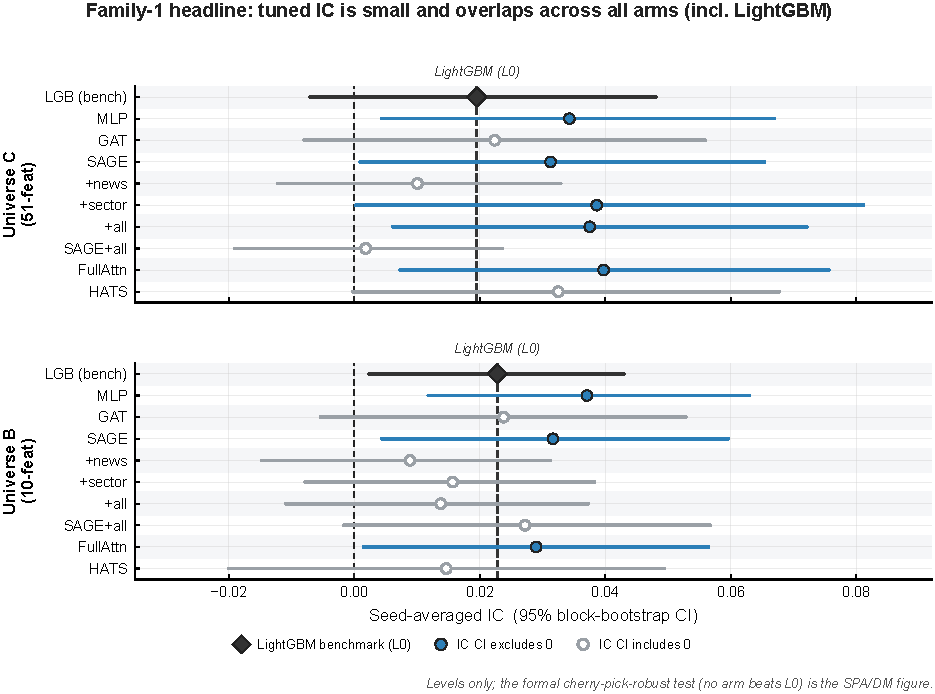
\includegraphics[width=\textwidth]{headline_ic_ladder}
  \caption{Per-arm pooled IC forest for the L0--L7 ladder in both universes, with the tuned LightGBM (L0) reference. \emph{Seeds${}=10$; folds${}=12$ (expanding walk-forward, 2023\,Q1--2025\,Q4); metric${}={}$pooled Spearman IC; intervals${}={}$95\% stationary block-bootstrap (block${}=21$\,d, 5000 reps); benchmark${}={}$L0.}
  \label{fig:headline}
\end{figure*}

\begin{table}[t]
  \centering
  \caption{Per-arm pooled IC with 95\% block-bootstrap CI. ``e0'' marks CI excluding zero.}
  \label{tab:ic}
  \small
  \begin{tabular}{@{}lccc c@{}}
    \toprule
    Rung & Univ B IC & e0 & Univ C IC & e0 \\
    \midrule
    L0 LightGBM & 0.0228 & y & 0.0195 & n \\
    L1 MLP      & 0.0371 & y & 0.0343 & y \\
    L2 GAT(corr)& 0.0238 & n & 0.0224 & n \\
    L2s SAGE    & 0.0317 & y & 0.0313 & y \\
    L3 +news    & 0.0089 & n & 0.0101 & n \\
    L4 +sector  & 0.0157 & n & 0.0386 & y \\
    L5 +both    & 0.0138 & n & 0.0375 & y \\
    L5s SAGE all& 0.0272 & n & 0.0018 & n \\
    L6 full-attn& 0.0290 & y & 0.0397 & y \\
    L7 HATS     & 0.0147 & n & 0.0325 & n \\
    \bottomrule
  \end{tabular}
\end{table}

\subsection{The predictive family: SPA and DM/HLN}\label{sec:spa}
Hansen SPA fails to reject ``no candidate beats LightGBM'' in both universes ($p_{\text{consistent}}=0.2767$ for B, $0.0774$ for C; $M=9$, $T=749$). Universe~C is the smaller $p$-value but does not reject at 5\%, and the comparison is underpowered, so this is a fail-to-reject. The cherry-pick-robust verdict is: no tuned arm is confirmed to beat tuned LightGBM. The local DM/HLN ladder under BH-FDR over the 20-test family tells a sharper story (Figure~\ref{fig:spa}, Table~\ref{tab:dm}). \emph{Within this tuned ladder}, the neural lift comes from the non-graph MLP and the graph does not add to it: in Universe~C the MLP beats LightGBM (L1$-$L0${}=+0.0148$, BH-reject) while the correlation-GAT loses to the MLP (L2$-$L1${}=-0.0119$, BH-reject), and the tuned news-edge arm loses to the correlation-GAT (L3$-$L2${}=-0.0123$, BH-reject). These are local ladder rungs, not a global ``graphs hurt'' claim: the sector, full-attention, HATS, and combined-edge arms all recover above the correlation-GAT in Universe~C, and the SPA non-rejection is the multiplicity-honest summary.

\begin{figure*}[t]
  \centering
  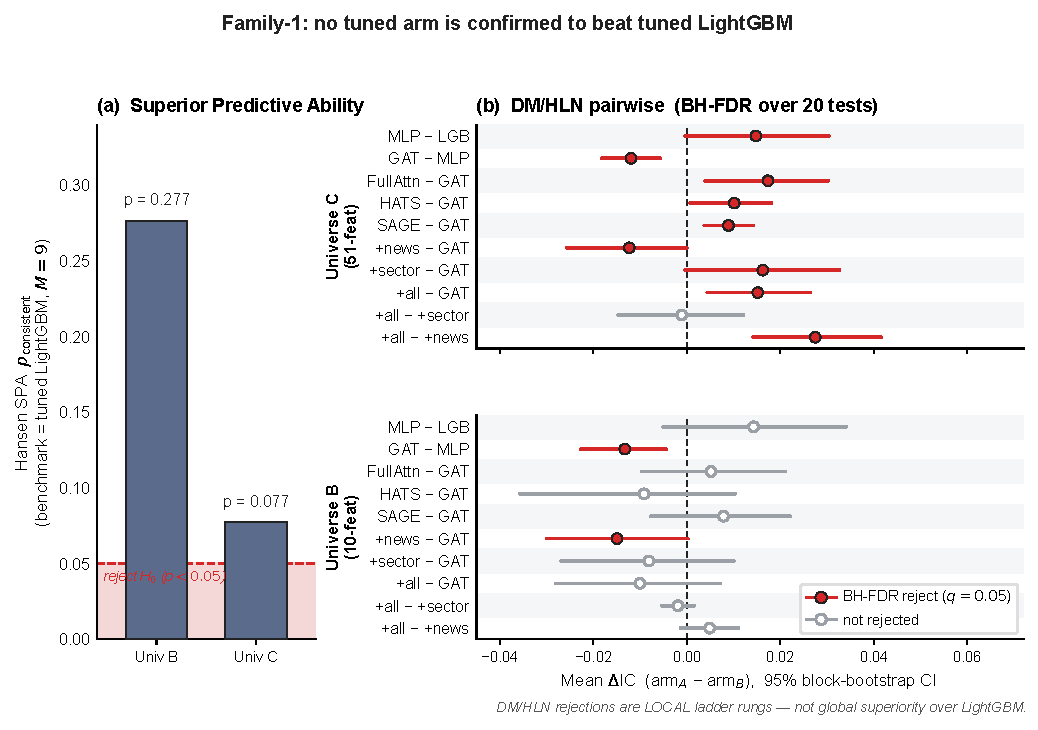
\includegraphics[width=\textwidth]{F9_spa_dm_confirmatory}
  \caption{Left: Hansen SPA $p_{\text{consistent}}$ per universe with the 5\% reject region shaded; neither universe rejects. Right: the 20 DM/HLN ladder rungs as a BH-FDR forest ($\Delta$IC${}\pm{}$CI), filled${}={}$BH-reject, hollow${}={}$not. \emph{DM/HLN with NW-HAC SE + HLN small-sample correction ($h=21$); BH-FDR $q=0.05$ over 20 tests; benchmark${}={}$L0.}
  \label{fig:spa}
\end{figure*}

\begin{table}[t]
  \centering
  \caption{DM/HLN pairwise ladder (seed-averaged daily $\Delta$IC; BH-FDR over the 20-test family). $r$ = BH-reject.}
  \label{tab:dm}
  \small
  \begin{tabular}{@{}l rc rc@{}}
    \toprule
    Pair (A$-$B) & B $\Delta$IC & $r$ & C $\Delta$IC & $r$ \\
    \midrule
    L1$-$L0 & $+0.0143$ & n & $+0.0148$ & y \\
    L2$-$L1 & $-0.0133$ & y & $-0.0119$ & y \\
    L6$-$L2 & $+0.0052$ & n & $+0.0174$ & y \\
    L7$-$L2 & $-0.0091$ & n & $+0.0102$ & y \\
    L2s$-$L2& $+0.0079$ & n & $+0.0089$ & y \\
    L3$-$L2 & $-0.0149$ & y & $-0.0123$ & y \\
    L4$-$L2 & $-0.0081$ & n & $+0.0163$ & y \\
    L5$-$L2 & $-0.0100$ & n & $+0.0152$ & y \\
    L5$-$L4 & $-0.0019$ & n & $-0.0011$ & n \\
    L5$-$L3 & $+0.0049$ & n & $+0.0275$ & y \\
    \bottomrule
  \end{tabular}
\end{table}

\subsection{Regime concentration}\label{sec:regime}
Pooled IC hides that cross-sectional skill is episodic. Figure~\ref{fig:regime} disaggregates IC by fold: skill is concentrated in a minority of quarters (notably 2024\,Q4 and 2025\,Q2), while roughly half the quarters sit near zero or negative for nearly every arm. A pooled IC is an average over a strongly non-stationary series; per-fold disclosure is mandatory, and any single-quarter Sharpe should be read with its period count.

\begin{figure*}[t]
  \centering
  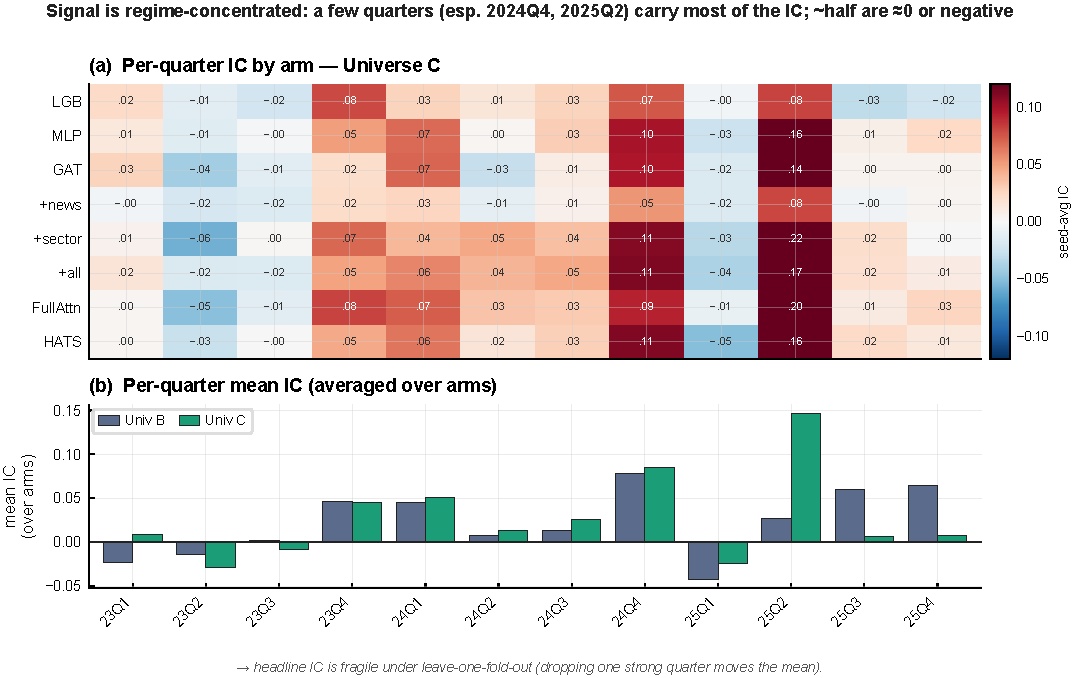
\includegraphics[width=\textwidth]{regime_perfold_ic}
  \caption{Per-arm $\times$ per-quarter IC heatmap (rungs $\times$ 12 folds) with a per-quarter mean-IC bar. \emph{Seeds${}=10$; folds${}=12$; metric${}={}$per-fold pooled Spearman IC.}
  \label{fig:regime}
\end{figure*}

\subsection{Net-of-cost crosswalk}\label{sec:cost}
Every pre-registered ranking claim is re-expressed under a 10\,bps net-of-cost convention (Table~\ref{tab:cost}, Figure~\ref{fig:cost}); IC remains the sole confirmatory metric. The two load-bearing Universe-C rungs survive net economics with CIs excluding zero. The economic separation behind the L1$-$L0 rung is in fact starker than the $+0.0148$ IC gap: tuned LightGBM's own net Sharpe at 10\,bps is negative ($-0.22$) while the MLP's is $+0.95$, though the paired net $\Delta$Sharpe erodes mildly with cost as the MLP pays down its higher turnover. The one cost-sensitive result is C L3$-$L2: the BH-significant IC underperformance of the news-edge rung versus corr-GAT does not carry to net Sharpe (net $\Delta$Sharpe${}=+0.08$, CI $[-0.77,+0.89]$ straddling zero, fold-fragile). The honest reading takes the net bootstrap CI as primary: the ranking-level underperformance does not reproduce economically, and this is a local IC rung, not a causal or economic statement that news edges help or hurt (Section~\ref{sec:causal}).

\begin{table}[t]
  \centering
  \caption{Gross/net crosswalk for the load-bearing Universe-C rungs.}
  \label{tab:cost}
  \small
  \begin{tabular}{@{}l r l c@{}}
    \toprule
    Pair & Gross $\Delta$IC (BH) & Net $\Delta$Sharpe@10\,bps [CI] & Carries? \\
    \midrule
    C L1$-$L0 & $+0.0148$ (r) & $+1.17\;[+0.36,+2.08]$ & yes \\
    C L2$-$L1 & $-0.0119$ (r) & $-0.72\;[-1.42,-0.10]$ & yes \\
    C L3$-$L2 & $-0.0123$ (r) & $+0.08\;[-0.77,+0.89]$ & no (CS) \\
    C L5$-$L3 & $+0.0275$ (r) & $+0.88\;[+0.12,+1.65]$ & yes \\
    \bottomrule
  \end{tabular}
\end{table}

\begin{figure*}[t]
  \centering
  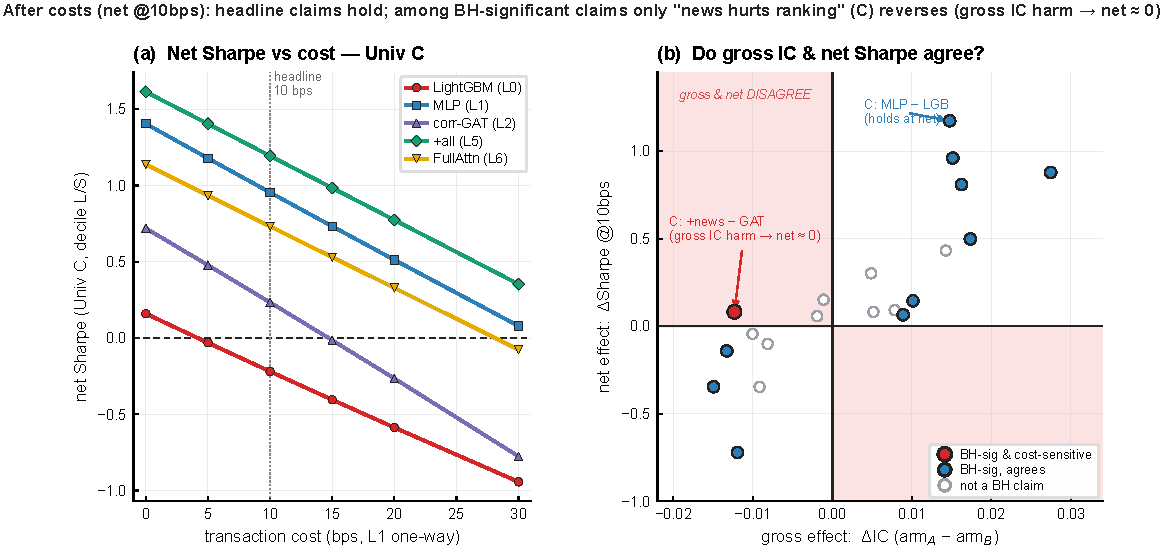
\includegraphics[width=\textwidth]{cost_gross_net}
  \caption{Left: the net-Sharpe cost ladder (0--30\,bps) for the Universe-C arms; tuned LightGBM (L0) is already negative at 10\,bps while the MLP (L1) stays positive. Right: gross-IC-vs-net-Sharpe sign agreement across the 20 pre-registered pairs, with the single sign-flip (C L3$-$L2) annotated. \emph{Net convention${}={}$10\,bps one-way on L1 turnover; per-pair net $\Delta$Sharpe${}={}$fold-level seed-averaged, stationary block bootstrap.}
  \label{fig:cost}
\end{figure*}

\subsection{The causal family: matched-capacity edges}\label{sec:causal}
Family-1's news-edge result confounds the edge with capacity. Family-2 removes that confound by running each edge set at the frozen L2 hyperparameter vector (Table~\ref{tab:family2}, Figure~\ref{fig:family2}). \textbf{0/6 contrasts survive BH-FDR and 6/6 are underpowered} ($|$matched $\Delta$IC$|<$MDE@80\%): edge effects are directionally positive but not family-significant, and fail-to-reject is not no-effect. The Universe-B reversals, matched $\Delta$IC positive where the tuned $\Delta$IC was negative, are evidence that the capacity confound masked a small positive edge effect at fixed capacity. In Universe~C the sector ($+0.0137$) and sector$+$news ($+0.0141$) contrasts agree in sign with their tuned counterparts, while the news contrast is small, positive ($+0.0011$), and opposite-signed to its negative tuned rung ($-0.0123$), so even the one edge that looked harmful on the tuned ladder is not harmful at fixed capacity.

\begin{table}[t]
  \centering
  \caption{Family-2 fixed-capacity edge contrasts (matched $\Delta$IC, BH-FDR over 6). UP${}={}$underpowered.}
  \label{tab:family2}
  \small
  \begin{tabular}{@{}ll r cc r@{}}
    \toprule
    Univ & Edge & Matched $\Delta$IC & BH & UP & Tuned $\Delta$IC \\
    \midrule
    B & news        & $+0.0015$ & n & y & $-0.0149$ \\
    B & sector      & $+0.0055$ & n & y & $-0.0081$ \\
    B & sector+news & $+0.0042$ & n & y & $-0.0100$ \\
    C & news        & $+0.0011$ & n & y & $-0.0123$ \\
    C & sector      & $+0.0137$ & n & y & $+0.0163$ \\
    C & sector+news & $+0.0141$ & n & y & $+0.0152$ \\
    \bottomrule
  \end{tabular}
\end{table}

\begin{figure}[t]
  \centering
  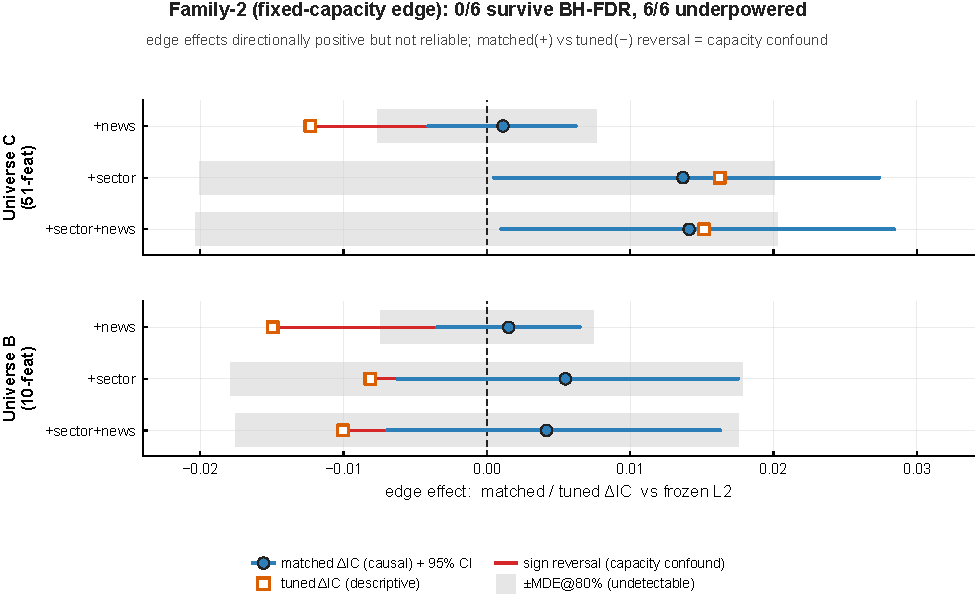
\includegraphics[width=\columnwidth]{family2_edge_causal}
  \caption{Matched-$\Delta$IC (causal) vs tuned-$\Delta$IC (descriptive) for the six edge contrasts, with the $\pm$MDE@80\% band; no contrast clears the band and none survives BH-FDR. \emph{Matched $\Delta$IC${}={}$fold-level seed-averaged at the frozen L2 HP vector, block bootstrap over 12 folds, BH-FDR $q=0.05$ over 6 contrasts.}}
  \label{fig:family2}
\end{figure}

\subsection{A tuned-config stability failure}\label{sec:stability}
One SAGE-Mean control arm under the full edge set in Universe~C (C/L5s) degenerates to a constant prediction in 27.5\% of its test fold-seeds (25 fully and 8 partially collapsed of 120). This is verified \emph{not} a training crash: the cells report a converged flag with a no-signal validation plateau, at which the cross-sectional Spearman IC is mathematically undefined. The mechanism is SAGE-mean aggregation over a dense edge set combined with the arm's tuned dropout of 0.5, which smooths the signal away, the same mechanism that explains why adding a correlation graph (L2) does not beat the MLP (L1). The arm is treated as missing (undefined IC $\neq$ a measured zero) and is never re-tuned, since re-tuning a single losing arm under an equal-budget design would be cherry-picking. The conclusion is invariant: under exclude/zero-fill/zero-skill the C/L5s mean IC stays ${}\approx0$ and the Universe-C SPA $p$ stays at $0.077$--$0.080$.

\subsection{Exploratory failure modes}\label{sec:exploratory}
These results sit outside the confirmatory families and are disclosed for transparency only. On a historical loss-function horse race (MSE was locked for the confirmatory ladder), ListMLE exhibited a systematic regime-shift inversion (Figure~\ref{fig:loss}): its per-cell mean IC is $-0.0458$ versus MSE's $+0.0113$. Its softmax-likelihood objective is dominated by the in-distribution rank order, so when test ranks shift the model produces anti-rankings. Separately, the Universe-C composition is the project's earlier Plan-AAA top-15 Alpha158 groups, originally ranked under a same-day-OHLC procedure; under strict $T-1$ leak correction only 5 of the top 15 stay in the top 15 (Figure~\ref{fig:planaaa}). Universe-C runtime features are evaluated at $T-1$ and are not leaked, but the basis for selecting them is fragile.

\begin{figure}[t]
  \centering
  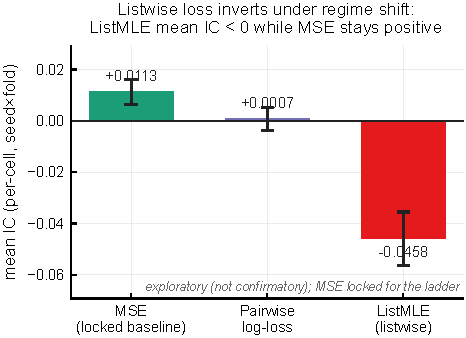
\includegraphics[width=\columnwidth]{loss_listmle_inversion}
  \caption{\emph{Exploratory (not confirmatory).} Mean IC per loss family on the historical loss horse race (per-cell, $\pm1$ SE); ListMLE inverts to a negative mean IC while MSE stays positive. MSE is the locked confirmatory loss.}
  \label{fig:loss}
\end{figure}

\begin{figure}[t]
  \centering
  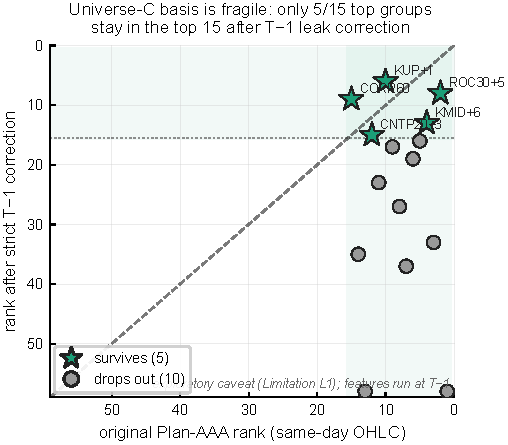
\includegraphics[width=\columnwidth]{plan_aaa_t1_stability}
  \caption{\emph{Exploratory caveat (Limitation L1).} Original Plan-AAA rank vs rank after strict $T-1$ correction for the top-15 Alpha158 groups; only 5/15 remain in the top 15. Runtime features are at $T-1$; only the composition basis is fragile.}
  \label{fig:planaaa}
\end{figure}

\section{Discussion}\label{sec:discussion}
A block-bootstrap CI tests a single point estimate against zero, whereas Hansen SPA asks whether the best of several candidates exceeds a benchmark after selection bias; both are correct and answer different questions. The headline is therefore not that GNNs fail, but that no tuned arm is \emph{confirmed} to beat a tuned tree benchmark on this span, and that the neural lift which does exist is MLP-shaped. In both universes the cleanest local DM rung is L2$-$L1${}<0$: adding a correlation-graph attention layer to the same features underperforms the plain MLP on IC, with the C/L5s collapse naming the candidate mechanism (aggregation over dense edges plus high dropout smooths the cross-sectional signal). This is a bounded statement about the correlation graph at the tuned operating point, not a general ``graphs hurt'' claim. Family-1's tuned news-edge rung looks like evidence that the news edge harms ranking, but Family-2 shows that at fixed capacity the same edge has a tiny, non-significant, and (in Universe~B) opposite-signed effect; equal-budget tuned ladders answer the deployment question, capacity-matched arms answer the scientific one, and conflating them is how edge-ablation claims get over-stated. Net economics does not rescue any edge; it confirms the one ranking-level edge effect was too small and too fold-fragile to be economically real.

\section{Limitations and Future Work}\label{sec:limits}
\textbf{(L1)} Universe-C's basis (Plan-AAA top-15) has low stability: only 5/15 groups survive $T-1$ correction (runtime features are at $T-1$; the basis is fragile). \textbf{(L2)} Skill is carried by a minority of the 12 quarters; report per-fold. \textbf{(L3)} The C/L5s constant-collapse is a reported stability finding. \textbf{(L4)} The vs-LightGBM comparison is underpowered (MDE exceeds the observed gaps), so ``no reliable evidence of superiority'', not ``proven equal''. \textbf{(L5)} Net Sharpe is descriptive, heavy-tailed and turnover-sensitive, so economic claims rest on fold-level paired $\Delta$Sharpe. \textbf{(L6)} L6 represents only the dense learned-attention family~\cite{li2024master,cheng2021adgat}, not learned-sparse graphs (e.g.\ FinMamba~\cite{finmamba2025}); LSTM/Transformer time encoders are not benchmarked. \textbf{(L7)} Single market and single horizon. Future work: replicate on 5+ years to dilute single-quarter dominance; cross-market replication; intra-day rebalance to target the short-window news signal that 21-day averaging removes; learned-sparse architectures under the same two-family protocol.

\section{Reproducibility}\label{sec:repro}
Code, the confirmatory run outputs, the frozen tuned hyperparameters (committed before launch), the three confirmatory analyzers, and the figure scripts are versioned in the project repository; a numeric-claim verifier is run on the working draft before each review. The pre-registered protocol and the two-family decision rules are fixed in a version-stamped protocol document.

%% --- Appendix: ST1 setup tables ---
\appendix
\section{Data and Experimental Setup (ST1)}\label{app:st1}

\begin{table}[h]
  \centering
  \caption{ST1a. Walk-forward fold calendar; pooled $T=749$ test days.}
  \label{tab:st1a}
  \small
  \begin{tabular}{@{}cc c cc@{}}
    \toprule
    Fold & Test quarter & Days & Fold & Test quarter / Days \\
    \midrule
    0 & 2023\,Q1 & 62 & 6  & 2024\,Q3 / 64 \\
    1 & 2023\,Q2 & 62 & 7  & 2024\,Q4 / 64 \\
    2 & 2023\,Q3 & 63 & 8  & 2025\,Q1 / 60 \\
    3 & 2023\,Q4 & 63 & 9  & 2025\,Q2 / 62 \\
    4 & 2024\,Q1 & 61 & 10 & 2025\,Q3 / 64 \\
    5 & 2024\,Q2 & 63 & 11 & 2025\,Q4 / 61 \\
    \bottomrule
  \end{tabular}
\end{table}

\begin{table}[h]
  \centering
  \caption{ST1b. Hyperparameter search grid (Optuna, $N=30$ per arm; centres${}={}$pilot defaults).}
  \label{tab:st1b}
  \small
  \begin{tabular}{@{}lll@{}}
    \toprule
    Dimension & Centre & Range \\
    \midrule
    \multicolumn{3}{@{}l}{\emph{Neural (MLP / GAT / L6 / L7)}}\\
    learning rate    & $10^{-3}$ & log-uniform $[10^{-4},10^{-2}]$ \\
    weight decay     & $10^{-4}$ & log-uniform $[10^{-5},10^{-3}]$ \\
    dropout          & 0.3 & $\{0.1,0.2,0.3,0.5\}$ \\
    hidden channels  & 64  & $\{32,64,128\}$ \\
    num layers       & 2   & $\{1,2,3\}$ \\
    attention heads  & 4   & $\{2,4,8\}$ \\
    \midrule
    \multicolumn{3}{@{}l}{\emph{LightGBM (L0)}}\\
    num leaves        & 31   & $\{15,31,63,127\}$ \\
    learning rate     & 0.05 & log-uniform $[0.01,0.1]$ \\
    min data in leaf  & 20   & $\{10,20,50,100\}$ \\
    $\lambda_{1},\lambda_{2}$ & $10^{-8}$ & log-uniform $[10^{-8},1.0]$ \\
    \bottomrule
  \end{tabular}
\end{table}

Fixed (not tuned): epochs${}=100$, patience${}=15$, gradient accumulation${}=32$; HATS relations${}=3$. The LightGBM grid is six-dimensional to match the neural dimension count and preserve an equal tuning budget. Ten canonical seeds: $\{7,34,86,99,123,456,789,1024,2024,2026\}$.

\bibliographystyle{ACM-Reference-Format}
\bibliography{references}

\end{document}
